\documentclass[a4paper,10pt]{article}

\usepackage{tikz}
\usepackage{fullpage}
\usepackage{amsmath,amsthm,amsfonts,amssymb,amscd}
\usepackage{mathtools}
\usepackage{colortbl}
\usepackage{xcolor}
\usepackage{graphicx}
\usepackage{titlesec}
\usepackage{xepersian}
\usepackage{multirow}
\usepackage{caption}
\usepackage{fancyhdr}
\usepackage{mdframed}


% ---------------------------
%      Color Palette
% ---------------------------
\definecolor{BgDark}{HTML}{141420}
\definecolor{BgCard}{HTML}{1E1E2E}
\definecolor{AccentBlue}{HTML}{7AA2F7}
\definecolor{AccentPurple}{HTML}{BB9AF7}
\definecolor{AccentCyan}{HTML}{7DCFFF}
\definecolor{AccentGold}{HTML}{E0AF68}
\definecolor{TextPrimary}{HTML}{CDD6F4}
\definecolor{TextMuted}{HTML}{6C7086}
\definecolor{RuleLine}{HTML}{313244}

\pagecolor{BgDark}
\color{TextPrimary}


% ---------------------------
%  RTL-safe Info Box
% ---------------------------
\newmdenv[
backgroundcolor=BgCard,
fontcolor=TextPrimary,
linecolor=AccentBlue,
linewidth=1.2pt,
rightline=true,   % RTL: accent border on the RIGHT
leftline=false,
topline=false,
bottomline=false,
innerrightmargin=12pt,
innerleftmargin=12pt,
innertopmargin=10pt,
innerbottommargin=10pt,
skipabove=10pt,
skipbelow=10pt,
]{infobox}
% ---------------------------
%        Font Setup
% ---------------------------
\settextfont{Vazir.ttf}[
    BoldFont = Vazir-Bold.ttf,
    Path = fonts/
]
\setlatintextfont{Vazir.ttf}[
    BoldFont = Vazir-Bold.ttf,
    Path = fonts/
]

% ---------------------------
%     Custom Adjustments
% ---------------------------
\renewcommand{\baselinestretch}{1.2}
\renewcommand{\thesection}{\arabic{section}}

% User-defined commands for homework info (adjust as needed)
\newcommand{\HomeworkNumber}{5}
\newcommand{\HomeworkDeadline}{1405/2/22}
\newcommand{\id}{\texttt{\detokenize{@rezamohmd}}}



\begin{document}

% ---------------------------------
%           Title Page
% ---------------------------------
\begin{titlepage}
	
	% Background decorations — right-side rectangle + gold horizontal line
	\begin{tikzpicture}[remember picture, overlay]
		% Right-side vertical rectangle (accent block)
		\fill[BgCard]
		([xshift=-2.2cm]current page.north east) rectangle
		(current page.south east);
		\draw[AccentGold!60, line width=0.8pt]
		([xshift=-2.2cm]current page.north east) --
		([xshift=-2.2cm]current page.south east);
	\end{tikzpicture}
	
	\vspace*{2.2cm}
	
	\begin{center}
		% Logo
		
\includegraphics[scale=1.05]{assets/fum-logo.png}\\[1.0cm]
		
		\textcolor{RuleLine}{\rule{8cm}{0.6pt}}\\[0.6cm]
		
		{\Huge \bfseries \textcolor{TextPrimary}{مبانی و کاربردهای هوش مصنوعی}}\\[0.4cm]
		
		\textcolor{RuleLine}{\rule{8cm}{0.6pt}}\\[0.4cm]
		
		{\large \textcolor{AccentCyan}{دانشگاه فردوسی مشهد}}\\[0.1cm]
		{\normalsize \textcolor{TextMuted}{گروه مهندسی کامپیوتر}}\\[0.2cm]
		{\normalsize \textcolor{AccentGold}{دکتر زارعی}}\\[1.6cm]
		{\normalsize \textcolor{TextMuted}{بهار 1405}}\\[0.2cm]
		
		% Homework number — simple, normal size
		{\normalsize \textcolor{TextMuted}{تمرین شماره}}
		{\large \bfseries \textcolor{AccentBlue}{\HomeworkNumber}}\\[1.4cm]
		
		% Deadline badge — gold border
		\setlength{\fboxrule}{0.8pt}%
		\fcolorbox{AccentGold!60}{BgCard}{%
			\begin{minipage}{7cm}
				\centering\vspace{5pt}
				\textcolor{AccentGold}{\bfseries مهلت تحویل: \HomeworkDeadline}
				\vspace{5pt}
			\end{minipage}
		}\\[0.8cm]
		
		% TA box — gold border
		\fcolorbox{AccentGold!60}{BgCard}{%
			\begin{minipage}{8cm}
				\centering\vspace{5pt}
				\textcolor{TextMuted}{مسئول تمرین:} \quad \textcolor{AccentCyan}{\id}
				\vspace{5pt}
			\end{minipage}
		}
	\end{center}
	
\end{titlepage}
% ---------------------------------
%          Instructions Page
% ---------------------------------
\clearpage

\vspace*{4pt}
\begin{center}
	\colorbox{BgCard}{%
		\begin{minipage}{\dimexpr\linewidth-2\fboxsep\relax}
			\centering
			\vspace{6pt}
			{\bfseries\large \textcolor{AccentGold}{دستورالعمل‌ها}}
			\vspace{6pt}
		\end{minipage}%
	}
\end{center}
\vspace{6pt}

\begin{infobox}
	دانشجویان محترم لطفا به موارد زیر توجه فرمایید:
	\begin{itemize}
		\itemsep0.4em
		\item
		تحویل تمرین‌ها فقط از طریق سامانه آموزش مجازی دانشگاه امکان‌پذیر است.
		\item
		تمرین‌ها باید دست‌نویس، خوانا و با استفاده از خودکار آبی یا مشکی و یا به صورت دیجیتالی با استفاده از قلم نوری نوشته شوند.
		\item
		از تمرین‌های حل‌شده دیگران استفاده نکنید. پیامدهای این کار با دانشجو می‌باشد.
		\item
		نوشتن جواب آخر به تنهایی نمره‌ای نداشته و تمام مراحل حل، مشمول نمره می‌باشد.
		\item
		به دلیل موعد از پیش تعیین‌شده تمرین‌ها و برنامه درسی، امکان تمدید تمرین وجود ندارد. همچنین ارسال تمرین پس از موعد تعیین‌شده نمره‌ای نخواهد داشت.
		\item
		نحوه نام‌گذاری فایل پاسخ باید مطابق جدول~\ref{tab:file_format} و به شکل \lr{\texttt{pdf}} باشد.
	\end{itemize}
	
	\vspace{10pt}
	
	% RTL-safe table: use center environment, manual column colors
	\begin{center}
		\arrayrulecolor{RuleLine}
		\begin{tabular}{|>{\columncolor{BgCard}\centering\arraybackslash}p{3cm}|>{\columncolor{BgDark}\centering\arraybackslash}p{7cm}|}
			\hline
			\textcolor{AccentCyan}{\bfseries\lr{Format}} &
			\texttt{\lr{StudentID-Full\_Name-\#HwNo.pdf}} \\
			\hline
			\textcolor{AccentGold}{\bfseries\lr{Example}} &
			\textcolor{TextMuted}{\texttt{\lr{9876543210-Alan\_Turing-\#01.pdf}}} \\
			\hline
		\end{tabular}
		\captionof{table}{\textcolor{TextMuted}{شیوه نام‌گذاری فایل‌ها}}
		\label{tab:file_format}
	\end{center}
	
\end{infobox}


\vspace{8pt}
\textcolor{AccentCyan}{\rule{\linewidth}{0.8pt}}
% ---------------------------------
%          questions
% ---------------------------------
%%%%%%%%%%%%%%%%%%%%%%%%%%%%%%%%%%%%%%%%%%%%%%%%%%%%%%%%%%%%%%%%%%%%%%%%%%%%%%%%%%%%%%%%%%%%%%
\section{\textcolor{AccentGold}{سوال اول}}

صحیح یا غلط بودن جملات زیر را مشخص کنید و توضیح کوتاه دهید.
\begin{enumerate}
	\item هر مسئله‌ی \lr{CSP} که \lr{path-consistency} در آن برقرار باشد، \lr{arc-consistency} هم در آن برقرار است.

	\item الگوریتم \lr{Forward Checking} می‌تواند تمام ناسازگاری‌های ممکن بین متغیرهای آینده را قبل از تخصیص آن‌ها تشخیص دهد.
	
	\item در یک \lr{CSP}، اگر یک متغیر فقط برای یک مقدار از دامنه‌اش با دامنه‌ی متغیر دیگر سازگار باشد، آن متغیر \lr{arc-consistent} در نظر گرفته می‌شود.
	
	\item استفاده از \lr{forward checking} در طول الگوریتم معادل با استفاده از \lr{AC3} قبل از اجرا و فیلتر کردن دامنه‌هاست.
	
	\item در مسئله‌ی \lr{Map Coloring} معمولاً قیود از نوع \lr{Binary Constraint} هستند.
\end{enumerate}

\bigskip
\textcolor{AccentCyan}{\rule{\linewidth}{0.4pt}}

\clearpage
%%%%%%%%%%%%%%%%%%%%%%%%%%%%%%%%%%%%%%%%%%%%%%%%%%%%%%%%%%%%%%%%%%%%%%%%%%%%%%%%%%%%%%%%%%%%%%
\section{\textcolor{AccentGold}{سوال دوم}}
\begin{enumerate}
	\item گرافِ محدودیتِ نشان‌داده‌شده در شکل شامل متغیرهای $A,B,C,D,E$ است که بین آن‌ها قیود همسایگی برقرار می‌باشد؛ به‌طوری‌که هیچ دو رأسِ مجاور نباید هم‌رنگ باشند. دامنه‌ی هر متغیر شامل سه رنگ \lr{r}, \lr{b}, \lr{g} است.
	
	می‌خواهیم این مسئله‌ی \lr{CSP} را با استفاده از الگوریتم جستجوی پسگرد (\lr{Backtracking}) و به‌کارگیری هم‌زمان تمام هیوریستیک‌های زیر حل کنیم:
	\begin{itemize}
		\item \lr{MRV}
		\item \lr{Degree heuristic}
		\item \lr{LCV}
		\item \lr{Forward Checking}
	\end{itemize}
	
	روند انتخاب متغیرها و تخصیص مقادیر را مرحله‌به‌مرحله نشان دهید و بیان کنید چگونه هیوریستیک‌ها در هر مرحله بر تصمیم‌گیری تأثیر می‌گذارند.
\end{enumerate}

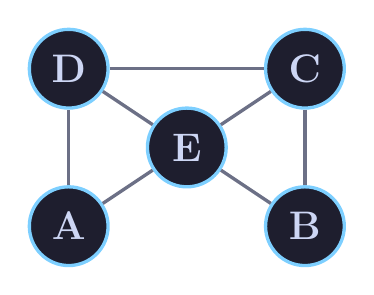
\begin{tikzpicture}[
	scale=1,
	transform shape,
	main node/.style={
		circle,
		draw=AccentCyan,
		fill=BgCard,
		text=TextPrimary,
		very thick,
		minimum size=1cm,
		font=\Large\bfseries,
		align=center
	},
	% Undirected Edge style
	edge/.style={
		draw=TextMuted,
		very thick
	}
	]
	
	% ================= NODES =================
	\node[main node] (E) at (0, 0) {E};
	
	\node[main node] (D) at (-1.5, 1) {D};
	\node[main node] (C) at (1.5, 1) {C};
	
	\node[main node] (A) at (-1.5, -1) {A};
	\node[main node] (B) at (1.5, -1) {B};
	
	% ================= EDGES =================
	\draw[edge] (A) -- (D);
	\draw[edge] (A) -- (E);
	\draw[edge] (D) -- (E);
	\draw[edge] (D) -- (C);
	\draw[edge] (C) -- (E);
	\draw[edge] (C) -- (B);
	\draw[edge] (B) -- (E);
	
\end{tikzpicture}

\bigskip
\bigskip
\textcolor{AccentCyan}{\rule{\linewidth}{0.4pt}}

%%%%%%%%%%%%%%%%%%%%%%%%%%%%%%%%%%%%%%%%%%%%%%%%%%%%%%%%%%%%%%%%%%%%%%%%%%%%%%%%%%%%%%%%%%%%%%
\section{\textcolor{AccentGold}{سوال سوم}}


	می‌خواهیم گراف زیر را با سه رنگ رنگ‌آمیزی نماییم، به‌طوری که هیچ دو رأس مجاور رنگ یکسانی نداشته باشند.
	اگر مقداردهی زیر انجام شده باشد:
	\begin{latin}
	V = \lr{red}, \qquad NT = \lr{red}
	\end{latin}

	این ناسازگاری با کدام یک از روش‌های زیر قابل تشخیص است؟
	\begin{enumerate}
		\item \lr{Forward Checking}
		\item \lr{Arc-Consistency}
		\item \lr{Path-Consistency}
	\end{enumerate}

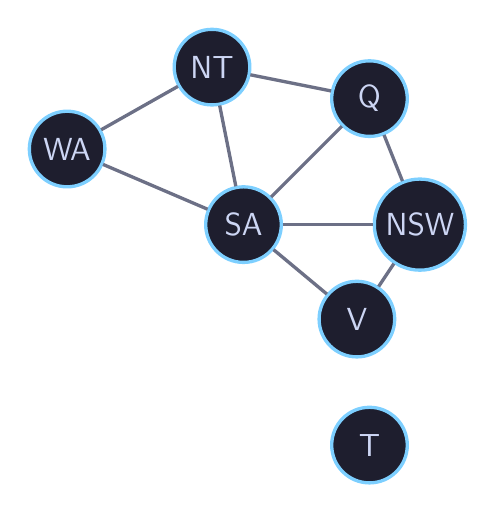
\begin{tikzpicture}[
	scale=0.8,
	transform shape,
	% Standard node style
	main node/.style={
		circle,
		draw=AccentCyan,
		fill=BgCard,
		text=TextPrimary,
		very thick,
		minimum size=1.2cm,
		font=\Large\sffamily,
		align=center
	},
	% Undirected Edge style
	edge/.style={
		draw=TextMuted,
		very thick
	}
	]
	
	% ================= NODES =================
	\node[main node] (SA) at (0, 0) {SA};
	
	\node[main node] (WA) at (-2.8, 1.2) {WA};
	\node[main node] (NT) at (-0.5, 2.5) {NT};
	
	\node[main node] (Q) at (2.0, 2.0) {Q};
	\node[main node] (NSW) at (2.8, 0) {NSW};
	\node[main node] (V) at (1.8, -1.5) {V};
	
	\node[main node] (T) at (2.0, -3.5) {T};
	
	% ================= EDGES =================
	\draw[edge] (WA) -- (NT);
	\draw[edge] (WA) -- (SA);
	
	\draw[edge] (NT) -- (SA);
	\draw[edge] (NT) -- (Q);
	
	\draw[edge] (SA) -- (Q);
	\draw[edge] (SA) -- (NSW);
	\draw[edge] (SA) -- (V);
	
	\draw[edge] (Q) -- (NSW);
	
	\draw[edge] (NSW) -- (V);
	
\end{tikzpicture}

\textcolor{AccentCyan}{\rule{\linewidth}{0.4pt}}
%%%%%%%%%%%%%%%%%%%%%%%%%%%%%%%%%%%%%%%%%%%%%%%%%%%%%%%%%%%%%%%%%%%%%%%%%%%%%%%%%%%%%%%%%%%%%%
\clearpage


%%%%%%%%%%%%%%%%%%%%%%%%%%%%%%%%%%%%%%%%%%%%%%%%%%%%%%%%%%%%%%%%%%%%%%%%%%%%%%%%%%%%%%%%%%%%%%
\section{\textcolor{AccentGold}{سوال چهارم}}

	یک جدول سودوکو \(4\times 4\) داریم که باید با اعداد ۱ تا ۴ پر شود به‌گونه‌ای که:
	\begin{enumerate}
		\item در هر سطر هیچ عددی تکرار نشود.
		\item در هر ستون هیچ عددی تکرار نشود.
		\item در هر بلوک \(2\times 2\) (زیرشبکه) هیچ عددی تکرار نشود.
	\end{enumerate}
	
	جدول اولیه به صورت زیر داده شده است:
	
	\begin{center}
		\begin{tabular}{|c|c|c|c|}
			\hline
			4 &   &   & 1 \\ \hline
			&  & 3  &   \\ \hline
			& 2 &  &   \\ \hline
			3 &   &   & 2 \\ \hline
		\end{tabular}
	\end{center}
	
	\textbf{الف.} این مسئله را به صورت یک \lr{CSP (Constraint Satisfaction Problem)} مدل کنید، به‌گونه‌ای که موارد زیر مشخص باشند:
	
	\begin{enumerate}
		\item مجموعه متغیرها (\lr{Variables}):  
		مشخص کنید هر خانه از جدول چه متغیری دارد و چگونه نام‌گذاری می‌شود.
		
		\item دامنه هر متغیر (\lr{Domains}):  
		دامنه مقادیر ممکن برای خانه‌های خالی و خانه‌های از پیش پر شده را تعیین کنید.
		
		\item مجموعه محدودیت‌ها (\lr{Constraints}):  
		محدودیت‌های مربوط به سطرها، ستون‌ها و بلوک‌های \(2\times 2\) را توضیح دهید.
	\end{enumerate}
	
	\textbf{ب.} با استفاده از روش \lr{Backtracking} توضیح دهید که:
	
	\begin{itemize}
		\item اولین متغیری که باید مقداردهی شود کدام است،
		\item اولین مقدار ممکن برای خانهٔ انتخاب‌شده چیست،
		\item و مسیر قدم‌به‌قدم اجرای \lr{Backtrack} چه خواهد بود.
	\end{itemize}
	
\bigskip
\textcolor{AccentCyan}{\rule{\linewidth}{0.4pt}}
%%%%%%%%%%%%%%%%%%%%%%%%%%%%%%%%%%%%%%%%%%%%%%%%%%%%%%%%%%%%%%%%%%%%%%%%%%%%%%%%%%%%%%%%%%%%%%



%%%%%%%%%%%%%%%%%%%%%%%%%%%%%%%%%%%%%%%%%%%%%%%%%%%%%%%%%%%%%%%%%%%%%%%%%%%%%%%%%%%%%%%%%%%%%%
\section{\textcolor{AccentGold}{سوال پنجم}}


	یک شرکت هواپیمایی قصد دارد ۶ پرواز را به سه گیت فرودگاه تخصیص دهد. هر پرواز باید از یکی از گیت‌ها انجام شود. بدیهی است دو پروازی که در یک بازه زمانی هستند نمی‌توانند از یک گیت استفاده کنند.
	
	\begin{center}
		\begin{tabular}{|c|c|c|}
			\hline
			\textbf{پرواز} & \textbf{مقصد} & \textbf{زمان} \\ \hline
			\lr{F1} & استانبول & 8--10 \\ \hline
			\lr{F2} & دبی       & 10--12 \\ \hline
			\lr{F3} & دوحه      & 9--11 \\ \hline
			\lr{F4} & مسقط      & 10--12 \\ \hline
			\lr{F5} & باکو      & 12--14 \\ \hline
			\lr{F6} & آنکارا    & 12--14 \\ \hline
		\end{tabular}
	\end{center}
	
	گیت‌ها: \lr{G1} ، \lr{G2} ، \lr{G3}
		\pagebreak
		
	\textbf{محدودیت‌ها:}
	\begin{itemize}
		\item گیت \lr{G1} برای هواپیماهای بزرگ مناسب نیست، بنابراین پروازهای \lr{F2} و \lr{F5} نمی‌توانند از این گیت استفاده کنند.
		\item گیت \lr{G2} به دلیل تعمیرات برای پرواز \lr{F3} قابل استفاده نیست.
		\item گیت \lr{G3} تنها یک هواپیما در بازه زمانی \lr{F1} دارد.
		\item پروازهای \lr{F3} و \lr{F4} توسط یک شرکت مشترک انجام می‌شوند و باید در یک گیت یکسان انجام شوند.
		\item پروازهای \lr{F6} و \lr{F2} نیز باید از یک گیت یکسان استفاده کنند.
	\end{itemize}
	
	\textbf{الف.} گراف محدودیت را رسم کنید.
	
	\textbf{ب.} مسئله را با روش \lr{Forward Checking} حل کنید و مراحل کاهش دامنه متغیرها را نشان دهید.
	
	\begin{center}
		\begin{tabular}{|c|c|c|c|c|c|}
			\hline
			\lr{F1} & \lr{F2} & \lr{F3} & \lr{F4} & \lr{F5} & \lr{F6} \\ \hline
			&        &        &        &        &        \\ \hline
		\end{tabular}
	\end{center}
	


\bigskip
\bigskip
\textcolor{AccentCyan}{\rule{\linewidth}{0.4pt}}
%%%%%%%%%%%%%%%%%%%%%%%%%%%%%%%%%%%%%%%%%%%%%%%%%%%%%%%%%%%%%%%%%%%%%%%%%%%%%%%%%%%%%%%%%%%%%%



% Add more sections as needed...

\end{document}
